\chapter{相关技术介绍}
\section{Spark平台介绍}
Apache Spark\cite{zaharia2010spark}是为了快速计算而设计出来的集群计算技术。它基于Hadoop MapReduce技术,并且扩展了Hadoop MapReduce模型来有效地进行更多类型的计算,包括交互式查询以及流处理。Spark最主要的特性是内存集群计算技术,将数据保持在内存而不序列化到硬盘上大大提高了计算速度。

Spark最早是由UC Berkeley的Matei Zaharia在2009年作为Hadoop的一个子项目进行开发的。它在2010年基于BSD整数开源并在2013年捐献给了Apache Software foundation(ASF)。从2014年的二月起,Spark已经成为了ASF中的顶级项目之一。Apache Spark官网将Spark定义为大规模数据处理的一个快速、通用的引擎。

Spark有如下主要特性
\begin{itemize}
    \item \textbf{速度快}。如果数据全部在内存中,Spark平台上的计算能比Hadoop MapReduce快100倍以上,如果数据在硬盘上,则能快10倍以上。
    \item \textbf{便于使用}。Spark支持Java/Scala/Python/R四种语言的API,提供了超过80多种高度抽象的操作来使得编写并行程序更加容易,并且提供了Scala,Python和R的交互式Shell用以快速熟悉验证想法。
    \item \textbf{通用性}。Spark联合了SQL、streaming和complex analytics。Spark由SQL and Dataframes, MLLib for machine learning\cite{meng2015mllib}, GraphX和Spark Streaming驱动。我们可以在同一个程序中无缝地联合使用这么多库。
    \item \textbf{随处运行}。Spark可以运行在Hadoop、Mesos、独立模式,还可以在云上运行。Spark可以访问包括HDFS、Cassandra、HBase和S3等在内的多种数据源。我们可以在独立集群模式下或者EC2或者Hadoop YARN或者Apache Mesos下运行Spark。访问位于HDFS、Cassandra、HBase、Hive、Tachyon和任何Hadoop数据源。
\end{itemize}

Spark有如下主要组成
\begin{figure}[ht]
\centering
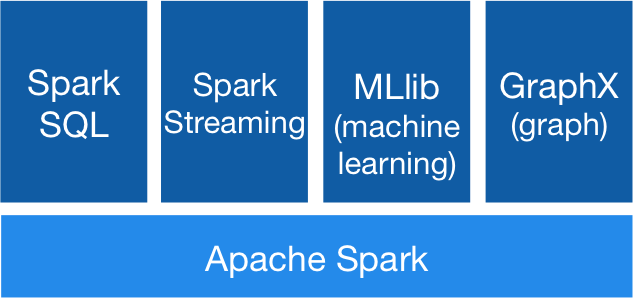
\includegraphics[width=10cm]{spark-stack}
\caption{Spark Stack}
\end{figure}
\begin{itemize}
    \item \textbf{Spark SQL}。Spark SQL使得你可以通过Java、Python、R、Scala语言在Spark程序中使用SQL或者熟悉的DataFrame API来查询结构化数据。并且DataFrames和SQL提供了一种通用的方式来访问多种不同的数据源,包括Hive, Avro, Parquet, ORC, JSON和JDBC。我们甚至可以使用对数据使用join操作。Spark SQL完全兼容Hive操作,我们可以对于已有的数据运行未经修改的Hive查询。通过JDBC和ODBC,我们可以使用标准的连接方式。
    \item \textbf{Spark Streaming}。Spark Streaming提供了Apache Spark语言级整合的API来进行流处理,我们可以像编写批处理任务的代码一样来编写流任务。支持java、Scala、Python。容错性较高,开箱支持从lost work和operator state中恢复。Spark整合性较好,可以把流处理和批处理以及交互式请求结合起来。
    \item \textbf{Spark MLlib}。Spark中的机器学习库,方便使用,MLlib可以和Python中的Numpy库进行交互,使用使用任何Hadoop数据源(HDFS, HBase or local files),使得MLlib很容易插入Hadoop workflow中。性能上,高质量算法,比MapReduce快100倍。方便部署,我们可以在Hadoop 2集群上不预装任何东西的情况下运行Spark和MLlib。
    \item \textbf{GraphX}。灵活性,可以在collections和graphs之间无缝整合,GraphX在单个系统中统一了ETL,解释分析,迭代图计算。我们我们把同一份数据视为graphs或者collections,transform或者join graphs。性能上,与其他专门的图处理系统相比是最快的。算法数量上,拥有很多图算法的实现,包括PageRand, Connected components, label propagations, SVD++, Strongly connected components, Triangle count等。
\end{itemize}

\subsection{Spark内部部署结构}
Spark中内部部署情况如图。
\begin{figure}[ht]
\centering
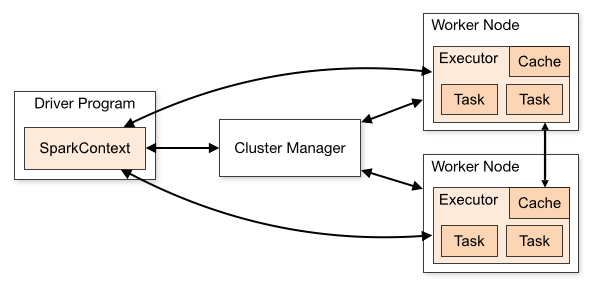
\includegraphics[width=10cm]{cluster-overview}
\caption{cluster overview}
\end{figure}
一个Spark集群,由初始化了SparkContext的驱动程序,和许许多多个工作节点组成。
我们把程序提交到Spark Driver上,由cluster manager来进行任务调度,实际的计算任务几乎都落在Spark Nodes上。由于任务调度的关系,Driver和Work Nodes最好能够在同一个局域网下,不然因为网络延迟以及带宽的缘故,花在网络等待的时间可能较长。
\subsection{Spark基本编程模型}
Spark中最基本的数据类型是RDD( Resilient Distributed Dataset)\cite{zaharia2012resilient}。它可以通过读取Hadoop InputFormat或者通过其他RDD Transform得到。在Spark中由两种最基本的操作transform和action,可以认为是MapReduce的扩展。

下面介绍一下我们的算法中用到的一些Spark提供的变换和操作。如表
\begin{table}[htbp]
\centering
\caption{Spark中的transformation操作} \label{spark:transform}
\begin{tabular}{|p{5cm}|p{10cm}|}
\hline
map(func)	& 对每个元素使用func操作之后返回新的RDD\\ \hline
filter(func)	& 过滤func操作结果为假的元素,返回新的RDD \\ \hline
flatMap(func)	& 与map相似,但是每个输入元素映射到0或多个输出元素 \\   \hline
sample(withReplacement, fraction, seed) &	使用给定的随机种子,对输入的数据进行给定比例的采样 \\ \hline
union(otherDataset)	& 返回输入数据与参数联合的新RDD \\   \hline
intersection(otherDataset) &	返回数据数据与参数交集的新RDD\\ \hline
distinct([numTasks]))	& 返回输入数据中不同元素的新RDD \\ \hline
groupByKey([numTasks])	& 对数据集(K ,V)对进行操作,返回(K, Iterable<V>)对。\\ \hline
reduceByKey(func, [numTasks]) & 当在(K, V)对上调用的时候,返回(K, V)对数据集。值V必须满足类型(V, V)=>V,然后用func函数进行聚合得到。\\ \hline
sortByKey([ascending], [numTasks])	 & 当K是可排序的,在(K, V)对数据集上调用该函数的时候,返回ascending指定的升序或者逆序排列的(K, V)数据集对。\\ \hline
join(otherDataset, [numTasks]) &	 当在类型为(K, V)和(K, W)的数据集上调用的时候,返回(K, (V, M))的数据集对。此外还有leftOuterJoin/rightOuterJoin/LeftOuterJoin \\ \hline
cogroup(otherDataset, [numTasks])	& 在数据类型(K, V) 和(K, W)上进行调用的时候, 返回(K, (Iterable<V>, Iterable<W>))数据集对。\\ \hline
cartesian(otherDataset)	 & 当在数据类型T和U上进行调用时,返回所有的(T, U)对。\\ \hline
\end{tabular}
\end{table}

\begin{table}[htbp]
\centering
\caption{spark中的action操作} \label{spark:action}
\begin{tabular}{|p{5cm}|p{10cm}|}
    \hline
    reduce(func) & Aggregate the elements of the dataset using a function func (which takes two arguments and returns one). The function should be commutative and associative so that it can be computed correctly in parallel.\\ 
    \hline
    collect() & Return all the elements of the dataset as an array at the driver program. This is usually useful after a filter or other operation that returns a sufficiently small subset of the data. \\
    count() &  Return the number of elements in the dataset.\\
    first() &  Return the first element of the dataset (similar to take(1)).\\
    take(n) & Return an array with the first n elements of the dataset.  \\
    takeSample(withReplacement, num, [seed]) & Return an array with a random sample of num elements of the dataset, with or without replacement, optionally prespecifying a random number generator seed.  \\
    takeOrdered(n, [ordering]) &  Return the first n elements of the RDD using either their natural order or a custom comparator.\\
    saveAsTextFile(path) & Write the elements of the dataset as a text file (or set of text files) in a given directory in the local filesystem, HDFS or any other Hadoop-supported file system. Spark will call toString on each element to convert it to a line of text in the file. \\
    saveAsSequenceFile(path) 
(Java and Scala) &  Write the elements of the dataset as a Hadoop SequenceFile in a given path in the local filesystem, HDFS or any other Hadoop-supported file system. This is available on RDDs of key-value pairs that implement Hadoop's Writable interface. In Scala, it is also available on types that are implicitly convertible to Writable (Spark includes conversions for basic types like Int, Double, String, etc).\\
    saveAsObjectFile(path) 
(Java and Scala) &  Write the elements of the dataset in a simple format using Java serialization, which can then be loaded using SparkContext.objectFile().\\
    countByKey() & Only available on RDDs of type (K, V). Returns a hashmap of (K, Int) pairs with the count of each key.  \\
    foreach(func) & Run a function func on each element of the dataset. This is usually done for side effects such as updating an Accumulator or interacting with external storage systems. 
Note: modifying variables other than Accumulators outside of the foreach() may result in undefined behavior. See Understanding closures for more details. \\
    \hline
\end{tabular}
\note{这里是表的注释}
\end{table}

通常来说,传递给Spark操作(例如map或Reduce)的函数是在工作节点上运行的。函数内的所有变量在所有节点上都是一份独立的拷贝。在远程工作节点上对于这些变量的修改不会反馈到驱动程序中。在工作节点上,支持通用的可读写的共享变量是低效的。虽然如此,Spark提供了两张有限的共享变量:broadcast variables和accumulators。Broadcast variables允许我们在每台机器上保持一个只读的变量,而不用随着任务下发变量。Accumulators是符合交换律的只能“添加”的变量,在Spark可以用来实现计数器或者求和等操作。

\section{推荐系统介绍}
推荐系统在现在的场景中越来越重要,由于信息的爆炸式增加,互联网上的商品数量也在不断的增加,但是用户能够浏览的信息和商品都是有限的,如何让用户浏览他们需要的东西成为商品/服务提供者所面临的一个问题,引起了人们对于推荐系统的研究。推荐系统最早是由美国明尼苏达大学的小组进行研究的,目前针对推荐系统的研究较为广泛,推荐系统的应用也较为普遍。目前的推荐系统主要可以分为个性化推荐系统与非个性化推荐系统。个性化会根据针对不同用户推荐不同的数据,而非个性化推荐系统考虑的因素没有用户。除了基于用户评分的推荐算法,推荐系统还有很多变种,比如基于用户显式评分的推荐系统,基于用户隐式评分的推荐系统,基于信任关系的推荐系统。在推荐系统中也很很多值得研究的问题,比如冷启动问题,如何防止恶意用户攻击推荐系统等。
% todo 比较基于内容过滤与协同过滤算法的优劣之处
\subsection{算法总览}
%todo 编写顺序算法
在目前的非个性化推荐系统中,主要的实现方法是对每个item用户可以进行点击upvote,upvote比较靠前的就可以排在比较靠前的位置,对于需要考虑时间因素的新闻推荐,会综合考虑upvote数和已经发布的时间,比如在Hacker New网站中,使用的推荐算法是这个链接部分的https://medium.com/hacking-and-gonzo/how-hacker-news-ranking-algorithm-works-1d9b0cf2c08d。比如在知名的reddit网站,推荐算法由如下的数学表示
$$    t_s = A - B$$
$$x = U - D$$
$$ y = 1 if x > 0$$
$$z = |x| if |x| \geq 1$$
\begin{equation}
f(t_s, y, z) = \log_{10}z + \frac{yt_s}{45000}    
\end{equation}

对于评论的推荐算法如下
\begin{equation}
    \frac{\hat{p}+\frac{z^2}{2n}\pm z\sqrt{\frac{\hat{p}(1-\hat{p})}{n}+\frac{z^2}{4n^2}}}{1+\frac{z^2}{n}}
\end{equation}
这两部分是比较成功的推荐系统。

对于个性化推荐算法推荐算法,主要有我们如下介绍的基于内容过滤和协同过滤两大类,我们将在接下来的章节详细介绍这一部分。

\subsection{基于内容过滤的推荐算法}
基于内容过滤的推荐算法,根据一个用户消费的商品与其他的商品的相似性来进行推荐。而商品之间的相似性是通过用户评分之外的信息来计算,适合于在能够获取商品较多的信息下使用。使用基于内容过滤算法的推荐系统,不会遇到冷启动问题。关键在于对描述商品的信息的选取,通常情况下我们会使用tags作为商品的信息描述,tags的添加可以通过人工录入或者机器学习的方式的录入。每个tags视为一个维度,这样我们可以将一个商品表示成依赖tags的一个向量,通过计算两个向量之间的相似性,我们可以得出商品之间的相关性。我们需要注意的几个问题有,商品之间的tags可能是同义tags,所以需要注意tags的选取。

基于内容过滤的推荐算法,避免了冷启动问题,不会有商品因为刚加入系统时候缺少用户评分而无法推荐给用户。并且这样相似性计算可以可以解释。

\subsection{基于邻域的推荐算法}
    \begin{table*}[htbp]
    \centering
    \caption{用户评分矩阵}
    \begin{tabular}{|c|c|c|c|c|}
        \hline
        & 物品1 & 物品2 & 物品3 & 物品4 \\ \hline
        用户1 & 2& ? & 3 & 4\\ \hline
        用户2 & ? &4 &  4 & 5\\ \hline
        用户3 & 6 & ?& 2 & ? \\ \hline
    \end{tabular}
    \end{table*}
    我们可以通过已经获取的评分部分,去计算未获取的评分。就像表中的问号的部分那样。

    \begin{equation}
       similarity(\vec{A}, \vec{B}) = cosine(\vec{A}, \vec{B}) = \frac{\vec{A} \cdot \vec{B}}{\lVert\vec{A}\rVert\ast\lVert\vec{B}\rVert}
    \end{equation}

\subsubsection{相似关系}
基于领域的推荐算法最重要的方法就是描述相似关系,对于物品的相似性的定义关系到计算时的权重分配,使用不同的相似性计量标准会带来有一定差异的相似性结果。常用的相似性关系计量如下表所示
\begin{table}[htbp]
\centering
\caption{相似性关系一览表} \label{tab:similarity}
\begin{tabular}{|c|c|c|c|}
    \hline
    measure & preprocess & norm & similarity\\
    \hline
    Cosine & $\frac{v}{\lVert v \rVert}$ & - & $dot_{ij}$ \\
    \hline
    Pearson correlation & $\frac{v - \bar{v}}{\lVert v - \bar{v} \rVert}$ & - & $dot_{ij}$ \\
    \hline
    Euclidean distance & - & $\hat{v}^2$ & $\sqrt{n_i - 2 \cdot dot_{ij} + n_j}$ \\
    \hline
    Common neighbors & $bin(v)$ & - &$dot_{ij}$ \\
    \hline
    Jaccard coefficient & $bin(v)$  & $\lVert \hat{v} \rVert $  & $ \frac{dot_{ij}}{n_i + n_j - dot_{ij}}$ \\
    \hline
    Manhattan distance & $bin(v)$ & $\lVert \hat{v} \rVert$ & $ n_i + n_j - 2 \cdot dot_{ij}$ \\
    \hline
    Pointwise Mutual Information & $bin(v)$ & $\lVert \hat{v} \rVert$ & $ \frac{dot_{ij}}{\lvert U \rvert} \log \frac{dot_{ij}}{n_in_j} $ \\
    \hline
    Salton IDF & $bin(v)$ & $\lVert \hat{v} \rVert$ & $ \frac{\lvert U \rvert \cdot dot_{ij}}{n_jn_j^2}(-\log\frac{n_i}{U})$ \\
    \hline
    Log Odds & $bin(v)$ & $\lVert \hat{v} \rVert$ & $ \log \frac{ \frac{ \lvert U \rvert \cdot dot_{ij} }{ n_jn_{j}^{2} } }{1 - \frac{ \lvert U \rvert \cdot dot_{ij}}{n_in_{j}^{2}}}$ \\
    \hline
    Loglikehood radio & $bin(v)$ & $\lVert \hat{v} \rVert$ &
    $\!\begin{aligned}[t]
    & 2\cdot (H(dot_{ij}, n_j - dot_{ij}, n_j - dot_{ij}, \\
    &\lvert U \rvert - n_i - n_j + dot_{ij}) \\
    &    - H(n_j, \lvert U \rvert - n_j) - H(n_i, \lvert U \rvert - n_i))
    \end{aligned} $\\
    \hline
\end{tabular}
\note{表的相似性关系及其数学表示}
\end{table}

\subsubsection{用户与用户之间的相似关系}
每个用户和其他用户之间的相似关系可以通过该用户给消费过的物品评分来计算。我们可以认为每个物品都是一个维度,每个用户都是在高维空间的一个向量。我们可以通过计算两个用户共同评分过的的物品的之间的夹角。通过夹角的大小我们来评估用户之间的相似性。当夹角超过90度的时候,我们认为用户之间存在负相关性。这种负相关性不需要出现在我们的用户的邻居中,需要剔除掉。

算法表示,顺序算法表示

\subsubsection{物品与物品之间的相似关系}
介绍计算相似性的时候,注意讲一下在相似性计算的时候,存在一个问题,就是如果一个item-item pair只有一个用户评分的话,那么他们之间的相似性必然为1,我们在计算相似性的时候,要去掉这种情况。
\subsection{ALS算法}
ALS算法\cite{Zachariah:2012hh}
ALS(Alternating least square) 最小交替二乘法,主要是利用近似的矩阵分解方法来在推荐系统中进行推荐。ALS算法属于隐式因子分解。我们把分解出的因子矩阵认为是描述了电影和用户特征的矩阵,与在基于内容的推荐中的显式做出区分,故称为隐式因子。
我们有用户$u$和$i$如下公式
$$
Q_{ui} = \begin{cases}
r  & \text{if user u rate item i} \\
0 & \text{if user u did not rate item i}
\end{cases}
$$
r是评分的真实数据。如果我们有$m$个用户$n$和物品,我们希望从评分矩阵中学习出代表电影的因素的矩阵。那就是,代表每个电影的因子向量,可以让我们在特征空间中表示这部电影。我们也希望学习出来能够表示用户的因子向量。对于电影分解出的矩阵$Y \in \mathbb{R}^{fxn}$(每部电影都是一列)和用户的因子矩阵$X \in \mathbb{R}^{mxf}$(每个用户是一个行向量)。但是,我们有两个未知的变量。因此,我们采用一种使用正则化的交替最小二乘法来进行求解。通过这样,我们先使用$X$来求解$Y$,再使用$Y$来$X$。通过足够次数的迭代,我们可以到达一个收敛点,此时矩阵$X$和$Y$都在迭代中不再改变,或者改变极小。虽然如此,在数据中有一个小问题。我们没有完整的用户数据,也没有完整的物品数据,这也是我们我们希望设计实现推荐系统的愿意。因此我们在更新过程中没有获取评分的的电影进行惩罚。这样我们仅仅依赖于用户已经评分过的电影的评分数据,而不用依赖于在推荐系统中还没有评分的数据。我们定义了一个权重$w_{ui}$如下
$$w_{ui} = \begin{cases}
0 &\text{if  } q_{ui} = 0 \\
1 & \text{ else} 
\end{cases}$$

现在我们需要定义我们的优化目标,定义损失函数(loss function)如下
$$J(x_u) = (q_u - x_u Y) W_u (q_u - x_u Y)^T + \lambda x_u x_u^T$$。
$$J(y_i) = (q_i - X y_i) W_i (q_i - X y_i)^T + \lambda y_i y_i^T$$
我们致力于优化这个函数。注意到我们加入了正则化系数来避免对于数据的过拟合(overfiting)。这个损失函数是由解的,我们可以不需要利用梯度下降的方法,而是直接求解来完成。解如下
$$x_u = (Y W_u Y^T + \lambda I)^{-1} Y W_u q_u$$
$$y_i = (X^T Wi X + \lambda I)^{-1} X^T W_i q_i$$
注意到这里$x_{u1}$和$x_{u2}$之间并无关系,这就使得我们可以在不同的机器上并行计算这些值。
$W_u \in \mathbb{R}^{nxn}$ 和
$W_u \in \mathbb{R}^{mxm}$都是对角矩阵。对于正则化系数的选择我们可以通过交叉验证来完成。
\subsection{计算Top-N推荐目标}
算法
%\IncMargin{1em}
%\begin{algorithm}[htbp]
%\SetKwData{Left}{left}\SetKwData{This}{this}\SetKwData{Up}{up}
%\SetKwFunction{Union}{Union}\SetKwFunction{FindCompress}{FindCompress}\SetKwFunction{Sim}{Sim}\SetKwFunction{WeightedSums}{WeightedSums}
%\SetKwInOut{Input}{input}\SetKwInOut{Output}{output}
%
%\Input{\begin{itemize}
%    \item $M$, the user-item rating matrix. Each $M_{u,i}$ element represents a rating and is either in $\mathbb{N}$ or empty.
%    \item $u$, the user we'd like to cimputer recommendations for.
%    \item $n$, the number of item recommendations to return, where $n \in \mathbb{N}$.
%    \item Sim(u,v), a user-defined function which computes the cosine similarity between two user vectors $u$ and $v$.
%    \item WeightedSums(u, S) a user-defined function which computes the predicted rating for each item prediction for a given user u.
%    \item TopNRecommendations($R_u, n)$, a user-defined function which worts the scoreed predictions and outputs the top n highest ranked items.
%\end{itemize}}
%\Output{$R_u(n)$, the top n recommendations for user u}
%\BlankLine
%\emph{something can be written here}\;
%\For{user $u \in M$}{
%        \If{$ u \neq v$}{
%        $S_{u, v} \leftarrow Sim(u,v)$ \;
%        }
%        \For{item $i \in M$}{
%            \If{$ u did not interact with i$}{
%                $R_u \leftarrow$ \WeightedSums($u, i, S_{u, v}$) \;
%            }
%        }
%}
%$R_u(n) = TopNRecommendations(R_u, n)$
%\caption{顺序算法1}\label{algo_disjdecomp}
%\label{alog:algorithm2}
%\end{algorithm}
%\DecMargin{1em}